\chapter{Appendix A - AIS Data Description}

In addition to the information required by the AIS standard, message data enriched with more information was used for the purpose of this thesis.
    
The fields of the original source AIS data of single entry (that represents a message) are described below.

\subsubsection{FID}
    The FID is the unique message identifier expressed as v4 UUID.
\subsubsection{MMSI}
    The \textbf{Maritime Mobile Service Identity} (MMSI) is a nine-digit number identifying the vessel or boat. Since it is always present is the field that is most frequently used to identify a vessel
\subsubsection{IMO}
    \textbf{IMO} stands for International Maritime Organization and it is another way to uniquely indentify a vessel or boat. Not all means of maritime transport comply to this standard and which is why some of the AIS messages do not have this field.
\subsubsection{Vessel Name}
    Name of the vessel.
\subsubsection{Callsign}
    A Call Sign is a unique identifier for a transmitter station on the boat. Of course, since a vessel can be equipped by more than one radio station, and since these stations can be interchanged between ships, there is no static correlation between call sign and ship.
\subsubsection{Vessel Type}
    This field describe a type of vessel based on a first classification: the purpose of the ship. \\
    Possible options: 'Tanker' 'Tug' 'Fishing' 'Other' 'Reserved' 'Cargo' 'Unknown' 'Dredging' 'Not Available' 'Military' 'SAR' 'HSC' 'Pilot' 'Towing' 'Vessel With Anti-Pollution Equipment' 'Diving' 'Port Tender' 'Pleasure Craft' 'Law Enforcement' 'Passenger' 'WIG' 'Sailing' 'Ships Not Party to Armed Conflict' 'Spare' 'Medical Transport'
\subsubsection{Vessel Type Code}
    Numeric version of the previous field.
\subsubsection{Vessel Type Cargo}
    Notes about cargo, if present.
\subsubsection{Vessel Class}
    Here is the class of vessel that help quantify the degree of seaworthiness of a boat based on the wave height and wind speed for which the boat is designed.\cite{vessel_classes}
    
    \begin{itemize}
    \item Category A: Ocean;
    \item Category B: Offshore;
    \item Category C: InShore;
    \item Category D: Inland or sheltered coastal waters.
    \end{itemize}

    
\subsubsection{Length}
    Length of vessel, in meters.
\subsubsection{width}
    Width of vessel, in meters.
\subsubsection{Flag Country}
    Country name of vessel flag.
\subsubsection{Flag Code}
    Country code of vessel flag.
\subsubsection{Destination}
    Destination of the trip of which the message is a part.
\subsubsection{ETA}
    This numeric field contains the Estimated Time of Arrival, expressed as the remaining estimated milliseconds to arrive at the destination.
\subsubsection{Draught}
    The Draught of a vessel measures the Maximum depth of any part of the vessel respect of the waterline, in meters. This determines the minimum depth of water a ship or boat can safely navigate. In some applications of analyzing these data, this value could be used as a proxy for the ship's cargo weight.
\subsubsection{Longitude}
    The current longitude according to the geographic coordinate system of the vessel.
\subsubsection{Latitude}
    The current latitude according to the geographic coordinate system of the vessel.
\subsubsection{SOG}
    Speed over Ground (SOG) is the speed of the vessel in one hour with respect to the land or any other fixed object such as buoys.
\subsubsection{COG}
    The Course Over Ground is the actual direction in degree of the motion considering the compensation for wind and current forces by changing the actual heading of the boat.
\subsubsection{ROT}
    Rate of turn indicator, indicates the rate a ship is turning in degrees per minute (°/min).
\subsubsection{Heading}
    The heading of a ship is a similar parameter to COG, since it too measures the direction of a ship. The heading is the compass direction the boat is pointing, and it may not match COG if there are current and tidal effects. Heading is instantaneous, COG can be derived from boat's motion over time.
    \\
    \begin{center}
    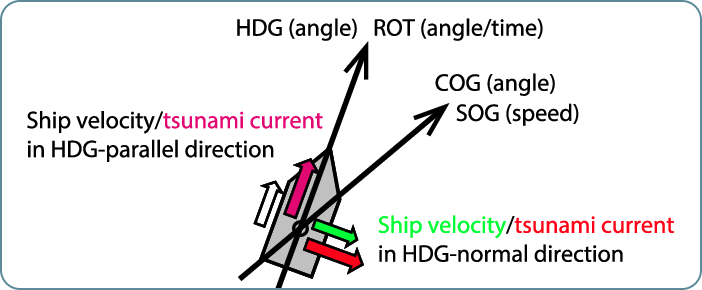
\includegraphics[width=10cm]{Images/1/cog-sog.png}
    \end{center}
    
\subsubsection{Nav Status}
    The status of the vessel. Possible options: \\'Under Way Using Engine' 'Engaged In Fishing' 'Not Defined' 'At Anchor' 'Restricted Manoeuvrability' 'Moored' 'Underway Sailing' 'Unknown' 'Not Under Command'.
\subsubsection{Nav Status Code}
    The status code of the vessel, related to the previous field.
\subsubsection{Source}
    This field describe the source of the message. The possible options are S-AIS and T-AIS.
    S-AIS stands for Satellite-based AIS.
    T-AIS stands for Terrestrial-based AIS.
\subsubsection{TS POS UTC}
    Datetime position in the format \verb|YYYYMMDDHHIISS|
\subsubsection{TS Static UTC}
    Datetime static in the format \verb|YYYYMMDDHHIISS|
\subsubsection{DT POS UTC}
    Datetime position in the format \verb|YYYY-MM-DD HH:II:SS|
\subsubsection{DT Static UTC}
    Datetime static in the format \verb|YYYY-MM-DD HH:II:SS|
\subsubsection{Vessel Type Main}
    Category of vessel. Possible options:\\ 'Oil And Chemical Tanker' 'Fishing Vessel' 'General Cargo Ship' 'Bulk Carrier' 'Gas Tanker' 'Tug' 'Service Ship' 'Offshore Vessel' 'Passenger Ship' 'Specialized Cargo Ship' 'Other' 'Pleasure Craft' 'Other Tanker'.
\subsubsection{Vessel Type Sub}
    Subcategory of vessel. Possible options:\\ 'Crude Oil Tanker' nan 'Lng Tanker' 'Pusher Tug' 'Research Vessel' 'Offshore Tug Supply Ship' 'Hopper Dredger' 'Refrigerated Cargo Ship' 'Dredger' 'Utility Vessel' 'Chemical Oil Products Tanker' 'Oil Products Tanker' 'Cruise Ship' 'Crane Ship' 'Icebreaker' 'Offshore Support Vessel' 'Nuclear Fuel Carrier' 'Landing Craft' 'Sailing Vessel' 'Patrol Vessel' 'Fish Carrier' 'Salvage Ship' 'Drilling Ship' 'Fish Factory Ship' 'Chemical Tanker' 'Fishing Support Vessel' 'Live Fish Carrier' 'Asphalt Bitumen Tanker'.
\subsubsection{Message Type}
    A numeric code that identifies the message type.